\documentclass[12pt, a4paper, oneside]{article}
\usepackage[utf8]{inputenc}
\usepackage{amsmath}
\usepackage{amsfonts}
\usepackage{amssymb}
\usepackage{fancyvrb}
\usepackage{verbatim}
\usepackage{makeidx}
\usepackage{graphicx}
\usepackage{color}
\usepackage{latexsym}
\usepackage{float}
\usepackage[pdftex=true,colorlinks=true,linkcolor=black,plainpages=false]{hyperref} % Suport hipertext
\usepackage[top=1.5in, bottom=1.5in, left=1.4in, right=1.4in]{geometry}

\setlength{\parskip}{4mm}%

\author{}
\title{
  \textbf{Message Passing Programming Coursework}\\
  MSc in High Performance Computing\\
  University of Edinburgh
}

\sloppy
\frenchspacing

%\begin{figure}[htbp]
% \centering
% \includegraphics[width=\textwidth]{plots/scale2}
% \caption{Loop 2 scalability with the selected scheduling}
% \label{figure:scale2}
%\end{figure}


\begin{document}
    \pagenumbering{gobble}
    \thispagestyle{empty}
	\maketitle
    \vspace{2cm}
    \tableofcontents
	\newpage
    \pagenumbering{arabic}


\section{Introduction}
In this project we aim to design, implement and test an application that executes an algorithm to reverse an edge-detection process in a grey scale image.
We want to parallelize this program using a message passing approach.
In concrete, we are going to use the MPI library, which has become the standard message passing library in HPC applications.

We do not only want a working solution but a well-structured, reliable and readable code, together with a set of correctness and performance tests. 
This will ensure the quality and the reproducibility of the applications as well as objective knowledge about its performance.
Each of these characteristics will be discussed in this project.

It is important to remark that all the data and figures presented in this project belongs to the last version of the code.
This has been possible thanks to the automatisation of all tests using scripts.
They were all run on the University of Edinburgh Morar cluster, which is a computer system with two nodes of 64 cores.
Each core has 2.2GHz and 10Mb of cache memory.
The language used in this project was Fortran90, and all tests were compiled with the PGI compiler with the flags \emph{-O3 -fastsse}
(some preprocessing was done with the gnu compiler using C-style directives).
The MPI implementation used in the tests was the MPICHv2.


\section{Design of the program }

Although we plan to implement the project using the MPI library, we designed the main program \emph{invertedges.F90} as a message passing library agnostic program.
It means that the main program calls message passing specific routines which are implemented in a specific fortran module.
Also the real numbers precision is abstracted of the main program to the \emph{precisiondef.F90} file.
Such approach enable us to improve the atomicity of the code and we can easily change the implementation we desire to use by changing the module imported.

The reverse edge-detection algorithm used is quite simple, it fundamentally iterates a specific number of times over this operation:
$$ new_{i,j} = 0.25 * (old_{i-1,j}+old_{i+1,j}+old_{i,j-1}+old_{i,j+1}+edges_{i,j}) $$
where the old array starts with all values at 255 and it is updated with the values of the new array at the end of each iteration.

The program should also be able to print out the average value of the pixels and check if a certain stopping criterion is satisfied at appropriate intervals.
The stopping criterion is based on the maximum change a pixel differs from the old array to the new one in a iteration.
When this maximum change is lower than a threshold, the program must stop.
In section 5 we present a detailed analysis about how many iterations represents an appropriate interval.

In order to parallelize the code we will use a domain decomposition pattern with halo swaps between each iteration.

To achieve all the described features, we have specified the following problem related routines that must be implemented in the message passing library dependent module:
\begin{itemize}
    \item Initialization: Define and initialize the needed data structures.
    \item Data distribution: Scatter the image data between all the processes.
    \item Halo swap: Send and receive appropriately the local array halos between the image neighbours. Also a function to know when the operation is completed.
    \item Get Average: Get the global average of the pixels from every process.
    \item Get Maximum change: Get the global maximum change from the old to the new array in any process.
    \item Gather data: Gather back all the data to the root process in order to write it to the output file.
    \item Finalize: Free the used resources.
\end{itemize}
Plus a set of useful operations whose implementation will depend on the message passing implementation used, such as: print once, print all, exit all and timing functions.

The project contains two implementations of this set of routines, one in a serial fashion, which can be found in the \emph{ieserial.f90} file, and a second one using the MPI library, in \emph{iempi.f90} file.

A build system was created to facilitate the compilation process of the application, it has two compilation entry points
(if none are specified, by default it creates the parallel version):
\begin{itemize}
    \item make serialversion: Creates a executable in \emph{binserial/invertedges} which uses the serial implementation module.
    \item make mpiversion: Creates a executable in \emph{bin/invertedges} which uses the MPI implementation module.
\end{itemize}

Finally, to execute the application we must use the following statement:
\emph{./binary input\_file \#iterations \#it\_btw\_reductions [output\_file]}
where the output file is an optional argument (if not specified it will be output.pgm) and the number of iterations must be set to 0 if we want to use the stopping criterion explained above. 
Note that in the MPI case, it must be preceded by \emph{mpiexec -n \#threads}.

\section{Implementation details}
The serial implementation only contains dummy routines, or local calculations without the messaging phases. Therefore, in this section we focus in the details of the MPI implementation.

In order to make the code simple and readable we have used most of the utilities which MPI provides. The principal ones are:
\begin{itemize}
\item We have created a cartesian communicator to locate all the processes in a 2-dimensional grid.
This representation fits quite naturally in our domain decomposition of the problem because we are managing an image represented as a 2D array.
The cartesian communicator also gives us the benefit to use the MPI suggested dimensions with the \emph{MPI\_dims\_create} routine.
And to easily find the neighbours of each process in both directions of the grid with the \emph{MPI\_cart\_shift} routine.

\item Another feature of MPI that we used is the derived datatypes.
This is because most of the sending/receiving operations we call during the program are not contiguous.
We have created the horizontal and vertical halos datatypes, the bock of data inside the halos, and the element of distribution in the root image, which we called masterblock.

\begin{figure}[htbp]
 \centering
 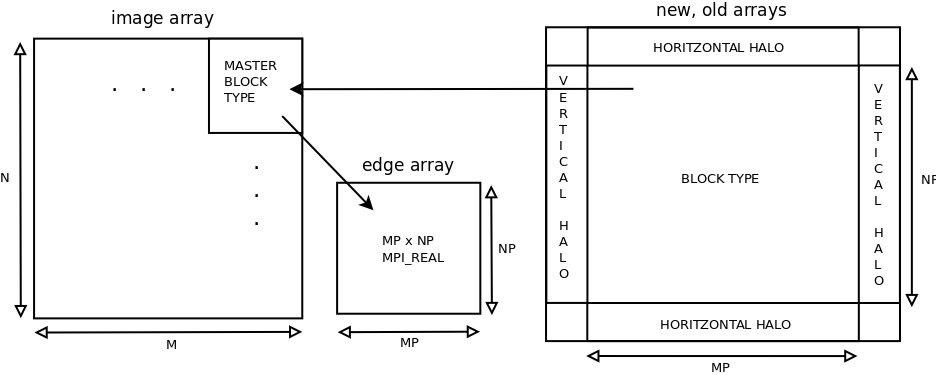
\includegraphics[width=\textwidth]{datatypes}
 \caption{Datastructures and MPI derived datatypes (sizes are not proportional).}
 \label{figure:datatypes}
\end{figure}

The usage of these datatypes allow us to eliminate intermidiate buffer data structures and describe the necessary MPI communications in a simple manner.

One may note that indeed, the horizontal halo has a contiguous memory layout, however, we have used this datatype to keep the code consistent and readable.

Also, we must be careful by the iterative usage of the masterblock in the collectives operations. To do them properly, we must resize the extent of the derived datatype and calculate the proper displacements to call the \emph{scatterv} and \emph{gatherv} routines.


\item We have implemented the sends and receives of the halo swaps using non-blocking communications. This decision was taken because they allow a common generic implementation for every process which is also deadlock free.
However, such approach also gives us the opportunity to perform some computation non dependent to the halos while they are being transmitted, hence hiding the communication time behind computation time.

A negative aspect of this approach is that we are not accessing the memory in a contiguos way, specially in the vertical halo dependent data, therefore, the advantages of the actual systems regarding memory locality optimization may be broken.

The best way to check if this improvement is practical is to implement both versions and profile the execution time of the algorithm (without IO times).
Doing so we obtain the results presented in table 1.%\ref{table:hiding}.

\begin {table}[H]
\centering
\begin{tabular}{|r|r|r|r|}
    \hline
               & Hiding & Not hiding & Percentual\\
     \#threads & communications & communications & difference\\
    \hline
    1  & 31.60 & 31.33 & -0.8 \% \\
    2  & 16.64 & 15.54 & -6.61 \% \\
    4  & 6.27 & 6.17 & -1.59 \%\\
    8  & 4.06 & 3.38 & -16.74 \% \\
    16 & 2.66 & 1.99 & -25.18 \%\\
    32 & 2.02 & 1.48 & -26.73 \%\\
    \hline
\end{tabular}
\label{table:hiding}
\caption{Time comparison between hidden and not hidden communications.}
\end{table}

The results show a clear time decrease in the code with not hidden communications and ordered memory access. Consequently, we have discarded the communication hiding implementation.
However, to allow us to investigate this option further in the future, we maintain the implementation of the halo swaps in two different routines: one for the non-blocking send/receives call operations and another to wait for those communications to be completed.

\end{itemize}

\section{Correctness Tests}
During the development of the project we took care of the quality of the code checking the reproducibility and the correctness of the results.

It is important to automatise those tests in order to execute them frequently and in every different system where we run the application. 
The main assurance that the code is working correctly for different input files and the number of processes is comparing the output of the parallel version with the output of the serial version(which should have a much more easier implementation).
Our project contains this correctness tests in the \emph{test/correctness/ctest.sh} script.

Due to the difficulties presented by parallel codes to be debugged, a frequent execution of these tests may be of great help to develop the code properly.

Nevertheless, we also applied some specific testing and debugging techniques in order to observe in closer level of details that we have the exact behaviour expected from the code.
Those techniques include the compilation of the code with \emph{-Wall -fbounds-check} flags during the development test.
Also the execution of some small specific input cases where we can print out the state of each array and manually compute that these values are correct.


Another tool which may give us valuable information about the proper behaviour of our application, as well as how it is performing, is a profiling data visualizer such as Vampire.

For instance, figure \ref{figure:complete} shows the profiling of the whole application executing 20 iterations of the algorithm with reduction operations every 5 iterations. This is a relatively small execution, therefore, the IO routines take a great amount of the execution time. For this reason the image has been cut to show the central part.
It is interesting to note that the first two iterations take a longer time than the rest because they are highly desynchronized, but after that, the iterations are relatively well balanced and in that zone the computation time is close to the 90\% of the total time.

\begin{figure}[htbp]
 \centering
 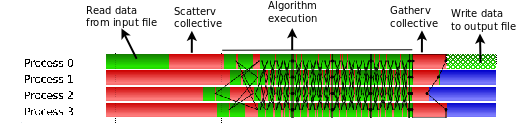
\includegraphics[width=\textwidth]{completemodif}
 \caption{Vampire visualization of the execution of the program.}
 \label{figure:complete}
\end{figure}

The following images show a detailed view of 5 iterations for the two different implementations proposed in the last section: the halo swaps communications hidden in some computation, in figure \ref{figure:detail1}, and all the communication steps at the beginning followed by all the computation, in figure \ref{figure:detail2}. It is also appreciable that the reduction operations are done every five iterations as stated in the execution command.

\begin{figure}[htbp]
 \centering
 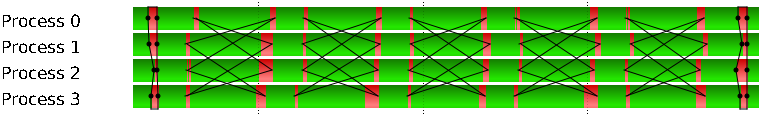
\includegraphics[width=\textwidth]{detailhiden}
 \caption{Detailed visualization of the communications hidden by computation.}
 \label{figure:detail1}
\end{figure}

\begin{figure}[htbp]
 \centering
 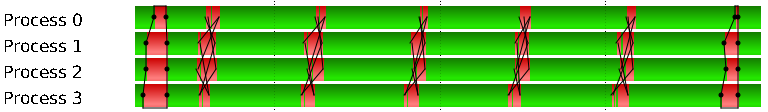
\includegraphics[width=\textwidth]{detailnothiden}
 \caption{Detailed visualization of the communications before the computation.}
 \label{figure:detail2}
\end{figure}




Finally, another important quality factor we must be concerned about is that we aim to create a standard compliant code in order to get a good portability.
For this reason we have compiled, executed and performed the correctness tests using different systems (my laptop, Morar and Hector), different compilers (gnu and pgi) and different MPI implementations (openMP and MPICHv2).
Most of these combinations are managed by the makefile commenting out the appropriate variables. As mentioned previously, the final version of the \emph{makefile} is ready to compile the program using the PGI compiler on Morar with the default MPI implementation of the system (mpif90).


\section{Performance Analysis}

One of the main goals, if not the most important, of every HPC application is to achieve good performance. For this reason, an extensive and accurate performance analysis is a major requirement for these kind of applications.

In order to obtain valuable and reproducible information about the performance, it is necessary to define a concrete execution environment (Morar with the defined flags in our case) and have all the tests automatized in scripts, like in the correctness case.
It is a great help to execute the application in a system such as Morar, where the process is not sharing the CPU cores with other processes at the same time. This reduces the amount of noise and randomness in the timing results.
However, to obtain even more stable results the average of 5 executions was taken.
Because in this project we are mainly interested in the execution and parallelization of the algorithm, in most of the experiments we got rid of the IO timing.

One of the application parameter introduced early in the report is the appropriate iteration separation between the reduction operations.
In order to find it, in our first test we performed many executions of 10000 iterations of the application with \emph{edge768x768.pgm} as input file.
In these executions we vary the iterations between the reductions. The results are presented in figure \ref{figure:reductions}.

\begin{figure}[htbp]
 \centering
 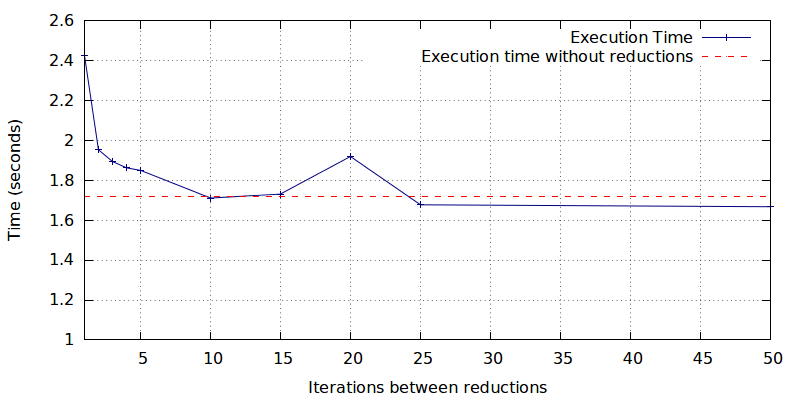
\includegraphics[width=\textwidth]{plots/reductions}
 \caption{Time variation changing reduction operations rate.}
 \label{figure:reductions}
\end{figure}

We can see how the execution time quickly decreases to a stable value around 1.7 seconds, the same time than the execution without any reduction. It approximately reach this stability in 10 iterations between reductions.

One of the typical information which is useful to know about in any algorithm is how the execution time grows when we increase the problem size.
For this concrete test, we have also analysed the IO reading and writing time because the input size may have a great impact in those operations.
The test is performed with 8 processes and 200 iterations of the algorithm, where only one reduction operation is performed.

\begin{figure}[htbp]
 \centering
 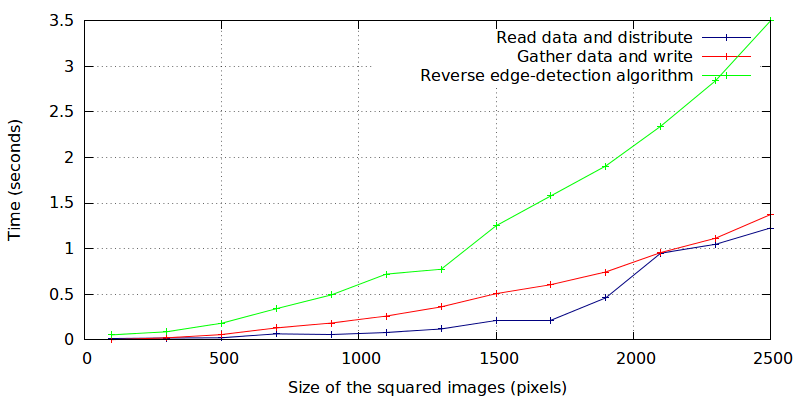
\includegraphics[width=\textwidth]{plots/imagesize}
 \caption{Execution time .}
 \label{figure:size}
\end{figure}

In this case, we can theoretically deduce that the implemented algorithm has a quadratic growth in both, the computation time and the memory needs.
This fact is confirmed in the figure \ref{figure:size}.
The figure also shows that the IO operations also grows with a similar tendency but in a smaller scale.
However, we note that they consume a significant amount of time and they will be a problem if we intend to increase the input size in higher ranks than the ones used in this project.

Finally, one of the key aspects of all parallel applications is to know how they scale in terms of the number of the processors used in the computation.
To represent this feature we have plotted in figure \ref{figure:scale} the execution time (left axis) of the application over a different number of processes, as well as the speed-up (right axis) obtained by those executions. The test is performed with 20000 iterations of the algorithm with reduction operations every 20 iterations.
In the speedup case, to achieve a good understanding of the values, the theoretically perfect speedup is also introduced to the plot.
\begin{figure}[htbp]
 \centering
 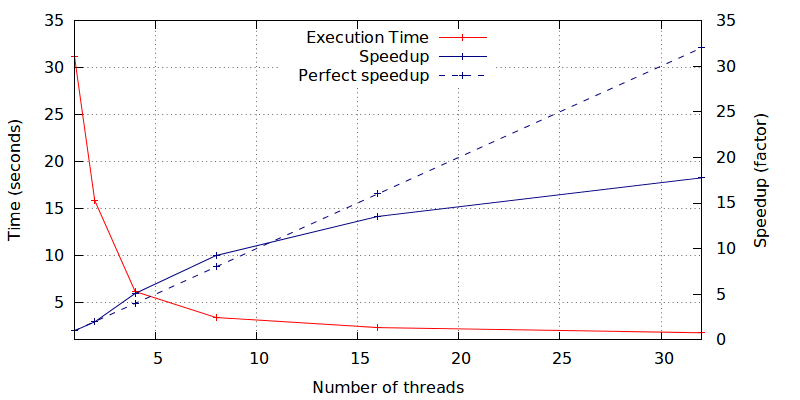
\includegraphics[width=\textwidth]{plots/scalability}
 \caption{Execution time and speedup in a scalability plot.}
 \label{figure:scale}
\end{figure}
The figure shows how the execution time decreases in a sharp rate in the first
part of the plot.  In fact we could note that the obtained speedup is better
than the theoretically perfect one.  Probably, it is due to some hardware
optimization, such the cache hierarchy, which is replicated on all the cores
added to the computation.  This may create an aggregated optimization effect.

However, from 12 processes on, the execution time, and consequently the speedup, keep decreasing their gains until stabilize around a 15 factor of speedup.
Further scaling has not been included to the plot because, from 32 threads on, the execution time remains approximately the same, or it is deteriorated.

This behaviour could have been produced by the fact that because we are performing a strong scaling test, the amount of data each process computes gets too small to be efficiently computed in a single process in comparison to the communications needed. However, we have tried the same test with bigger input files and the same behaviour has been found.
Therefore, we could conclude that the scaling reaches a limit produced by some physical system limitation or an implementation inherent limitation.
 


\section{Conclusions}

During the development of this project most of the MPI utilities and characteristics have been attempted in order to use the library as extensively an appropriately as possible.
We could ascertain that this problem, as well as any problem which might be parallelized using a domain decomposition, are very nicely handled by the MPI set of routines.
This leads to a natural and simple representation of the domain decomposition problems in MPI, which constitutes a good aspect in order to achieve a readable and easily debbugable code.

Nevertheless, we have experimented the big importance of assuring those quality factors from an early stage of the development. Some of the bugs encountered have been really difficult to debug due to the complexity of the runtime in parallel applications. Also, some of them where difficult to spot because they were only present under a certain compiler and/or systems.

For this reason, it has been essential to create a proper correctness test, and execute them frequently in the different environments when a new feature was introduced to the code.

It was also interesting to think about how to atomize the code in order to abstract the message passing library and real type precision from the main application.
This has been particularly useful late in the project when we compared the execution time of the serial and the parallel version.

Finally, the performance analysis part of the project has been useful to realize that every parameter in the code could have a big impact on the total performance, caused by the iterative behaviour of these kind of applications.
But maybe the most important observation was to realize how difficult it might be to scale an application over a certain number of processors, even though domain decomposition problems seem to have a good parallelization potential.

\end{document}
